\section{Context}
For the last ten years, Montefiore has been participating in a robotic contest named \emph{Eurobot}, where wheeled robots battle each other for points in various play environments. After some success, it was decided to move on to a more difficult contest, \emph{Robocup}.

This contest is quite vast and divided into several categories :
\begin{itemize}
\item Robocup Rescue : a category where robots are must perform various rescue operations in diverse scenarios.
\item RoboCup Industrial : a category with industrially oriented competitions.
\item RoboCup@Home : a league for domestic robots. This category has a social aspect to it.
\item RoboCupJunior : more of an initiative that aims to foster robotics interest in children rather than a contest, it helps organize various robotics events for younger minds.
\item RoboCup Soccer : historically the first category, centred about humanoid robots playing football in small teams. The objective of this category is to have a team of robots beat the world champions by 2050. This is the league we will compete in.
\end{itemize}
Robocup Soccer is further subdivided into 4 sub-categories :\begin{itemize}
\item Standard platform, where the teams all use the same robot(Nao).
\item Adultsize, for the taller robots
\item Teensize, for middle sized robots
\item Kidsize, for the smaller robots.
\end{itemize}

This year's team is preparing to participate to the Kidsize subcategory of the Robocup Soccer category. This master thesis is the by-product of that team's activity.

\begin{figure}[htp]
\center
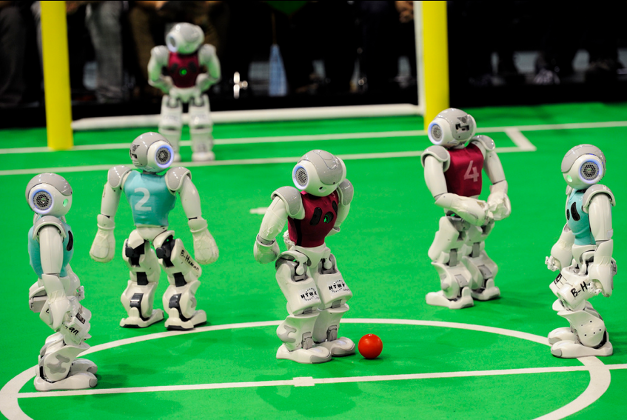
\includegraphics[width=0.5\textwidth]{figures/robocup}
\caption[Robocup Soccer standard platform]{Two teams of Nao robots playing against each other in the 2014 edition of RoboCup Soccer standard platform league\textit{[Photo courtesy of RoboCup]}}
\label{fig:intro_robocup}
\end{figure}

Since Montefiore is participating for the first time we are nearly starting from scratch and we don't really know how to build a good humanoid robot. In order to not spend countless hours building and testing different designs we need a tool able of simulating the physics
of a robot model. 

In particular, we want to use it to :
\begin{enumerate}
\item Test different robot designs and choose the best one, faster than it would be done by building the designs in real life.
\item At a later stage, be able to test control algorithms faster because the real robot is not needed.
\end{enumerate}

\section{Goals of the project}
The goal of this thesis is to provide the team with a simulation tool that provides the following features :
\begin{itemize}
\item realistically simulate the physics of objects including inertias, frictions, collisions and more.
\item receive and process orders incoming at a relatively high frequency. The processing need not be in real-time.
\item we want to use this simulator to test the code that would run on the real robot. That is, the simulator should provide the same interface to the code as the robot would.
\item visualize the results of the simulation.
\end{itemize}

\section{Structure of the report}
This report begins with an overview of the basics of physics simulation on computers before moving to the chapter that motivates the choice of V-Rep as the main simulation tool for this project.

Then, an in-depth presentation of V-Rep and Blender will be made in \cref{tools}, before detailing some experiments that were made to verify and improve the accurateness of the model.

\Cref{simulation} goes into the core of the subject with some simulations that influenced the design of the robot before being used to explore control strategies.

The last chapter will conclude the work by summing up and laying out future prospects.